\chapter{空间相干、van Cittert--Zernike 与强度干涉}
\label{chap:e10}

\begin{chapteropening}
第 \ref{chap:e09} 章讲的是"时间版"的相干：同一束光，此刻和稍后一会儿，还记不记得自己的相位。这一章把同样的问题搬到空间里去问。想象两台望远镜，相隔几十米、几百米，甚至几公里，同时盯着夜空里同一颗星。它们各自接到的光，是不是"同一个波前上的两小块"？如果是，两路强度会一起明、一起暗，涨落同步；如果这颗星在天上张开的角度大到一定程度，两台望远镜采到的就是波前上已经"错开"的两块，涨落各走各的，不再同步。神奇的是，同步程度的高低，直接告诉我们这颗星有多大——哪怕它在最大的光学望远镜里也只是一个点。本章要把这条链子一环一环接起来：先用纯几何算出"两台望远镜看到多细的角结构"，再用 van Cittert--Zernike 定理把"天空的样子"翻译成"相干度"，然后借第 \ref{chap:e08} 章的 Siegert 关系，说明为什么\emph{不用把两束光合到一起、只比较各自强度的抖动}就能测出恒星的大小。最后我们会碰到强度干涉的软肋——相位丢了——以及它作为交换换来的好处：几乎不怕大气抖动。
\end{chapteropening}

\section{几何：两台望远镜、一条基线、一个角尺度}
\label{sec:e10-geometry}

先把相关器、光子、量子统计统统放一边，只看一件几何事实——这件事连相机都用不上，一根尺子和一点三角就够了。

来自天空某个方向的星光，在离我们足够远的地方，波前已经拉平成一张几乎笔直的平面（这就是"远场"）。设这颗星在天上的方向由单位矢量 \(\bm s\) 指定。两台望远镜分别站在位置 \(\bm x_1\) 和 \(\bm x_2\)，它们之间的连线矢量叫\textbf{基线}（baseline）：
\[
  \bm B=\bm x_2-\bm x_1 .
\]
同一张平面波前先扫过一台望远镜，再扫过另一台，走的路程不一样。这段\textbf{程差}（path difference）等于把基线投影到星光传播方向上的长度，也就是点积 \(\bm B\cdot\bm s\)。真正对干涉有意义的，是垂直于视线、"贴在天空平面上"的那部分基线，记作投影基线 \(\bm B_\perp\)；沿视线方向的分量只是让整张波前整体早到或晚到，不改变两台望远镜看到的横向结构。

现在把注意力放在"星不是一个点、而是一小片天空"这件事上。取星面中心方向为 \(\bm s_0\)，在垂直于视线的\emph{局域天空平面}里架两个正交单位方向 \(\hat{\bm e}_x,\hat{\bm e}_y\)（分别对准基线两分量的方向）。星面上任意一点相对中心偏一个小角度，用两个小角坐标 \((l,m)\) 标记这个横向偏置（\(l,m\) 都以弧度计，量纲为一，典型值是 \(10^{-9}\) 弧度量级，也就是毫角秒）。那么这一点的方向可写成
\[
  \bm s\approx\bm s_0+l\,\hat{\bm e}_x+m\,\hat{\bm e}_y ,
\]
其中在小角一阶近似下 \(\bm s\) 仍近似归一（横向偏置只在二阶 \(\mathcal O(l^2,m^2)\) 上改变 \(|\bm s|\)，可忽略）。它带来的额外程差里，与中心不同的那部分就是
\[
  \Delta(\bm B\cdot\bm s)=B_x\,l+B_y\,m ,
\]
其中 \(B_x,B_y\) 是投影基线 \(\bm B_\perp\) 在天空平面两个正交方向上的分量（单位：米）。程差除以波长 \(\lambda\) 再乘 \(2\pi\)，就是这一点给两台望远镜带来的相位差。于是我们自然地定义一对\textbf{空间频率}（spatial frequency）：

\begin{equation}
  u=\frac{B_x}{\lambda},\qquad v=\frac{B_y}{\lambda}.
  \label{eq:e10-uv}
\end{equation}
\begin{formulaexplain}
\(B_x,B_y\)：投影基线在天空平面两方向上的分量（米）。\(\lambda\)：观测波长（米）。\(u,v\)：以"波长数"计的空间频率，量纲为一。同一条基线在越短的波长下，采到越细的角结构。
\end{formulaexplain}

为什么把它叫"空间频率"，而不直接叫"分辨率"？因为 \(u,v\) 数的是"这条基线上，横跨一个波长要放下多少条纹"。它是傅里叶平面上的一个采样坐标，不是角分辨率本身。代进真实数字感受一下：取 \(B=100\,\mathrm{m}\)、\(\lambda=500\,\mathrm{nm}=5\times10^{-7}\,\mathrm{m}\)，
\[
  \frac{B}{\lambda}=\frac{100}{5\times10^{-7}}=2\times10^{8}.
\]
两亿——这是个纯数字，表示这条基线横跨了两亿个波长。要得到角尺度，得把它\emph{倒过来}：
\[
  \frac{\lambda}{B}=\frac{1}{2\times10^{8}}=5\times10^{-9}\ \mathrm{rad}.
\]
把弧度换成毫角秒（\(1\,\mathrm{mas}=4.848\times10^{-9}\,\mathrm{rad}\)）：
\[
  5\times10^{-9}\,\mathrm{rad}=\frac{5\times10^{-9}}{4.848\times10^{-9}}\,\mathrm{mas}\approx1.0\,\mathrm{mas}.
\]
所以一条百米基线、蓝绿光，天生对应大约 1 毫角秒的角尺度——这已经比最好的单口径望远镜（衍射极限几十毫角秒）细几十倍。这就是干涉的全部魅力：分辨本领由\emph{望远镜之间的距离}决定，不由镜面口径决定。

\section{一阶空间相干度：跨望远镜的一支复箭头}
\label{sec:e10-gamma12}

几何告诉我们"这条基线对应多细的角结构"，但没告诉我们"这颗星在这个角尺度上究竟被分辨了没有"。要回答后者，必须比较两台望远镜真正接到的场。

回忆第 \ref{chap:e01} 章：某一时刻某一点的光场，可以写成一支在复平面里旋转的箭头——复振幅（complex amplitude）\(\mathcal E\)，它的长度是振幅、角度是相位。现在两台望远镜各有一支箭头 \(E_1(t)\) 和 \(E_2(t)\)。要问它们"步调多一致"，最自然的量是把一支箭头共轭后与另一支相乘再做时间平均，并用各自强度归一化。这个量叫\textbf{一阶空间相干度}（first-order spatial coherence，也叫复可见度）：

\begin{equation}
  \gamma_{12}^{(1)}
  =\frac{\big\langle E_1^{\ast}(t)\,E_2(t)\big\rangle}
        {\sqrt{\big\langle|E_1(t)|^2\big\rangle\,\big\langle|E_2(t)|^2\big\rangle}} .
  \label{eq:e10-gamma12}
\end{equation}
\begin{formulaexplain}
\(E_1,E_2\)：两台望远镜接到的复场。分子 \(\langle E_1^{\ast}E_2\rangle\) 是"跨望远镜的场相关"，分母把各自平均强度开方后归一化。结果 \(\gamma_{12}^{(1)}\) 是复数：模 \(|\gamma_{12}^{(1)}|\in[0,1]\) 给相干强弱，辐角给傅里叶相位。
\end{formulaexplain}

逐个符号说清楚。\(E_1(t),E_2(t)\)：两台望远镜同一瞬间接到的电场复振幅（在 CGS 里量纲是 \(\mathrm{statvolt\,cm^{-1}}\)，不过归一化后单位全约掉了）。角括号 \(\langle\cdot\rangle\) 是对时间的长时间平均。分母里 \(\langle|E_1|^2\rangle\) 正比于第一台望远镜的平均强度，开方后与第二台相乘，恰好把两路强度的绝对标度除干净，所以 \(\gamma_{12}^{(1)}\) 只反映"步调"，与两台望远镜谁收得多谁收得少无关。

为什么要用复数而不是一个实数？因为"步调一致"这件事本身有两层信息：\emph{有多一致}（模）和\emph{差了多少相位}（辐角）。振幅干涉仪（第 \ref{chap:e09} 章那种把两束光用延迟线合到一起看条纹的仪器）能把这支复箭头的模和辐角都读出来——条纹的对比度给模，条纹的位置给辐角。而本章后面要讲的强度干涉仪\emph{不}在光学上合束，它在探测之后比较两路强度的抖动，最后只拿到 \(|\gamma_{12}^{(1)}|^2\)，辐角丢了。这个"丢相位"是强度干涉的核心特征，我们第 \ref{sec:e10-phase} 节专门算账。

那么 \(\gamma_{12}^{(1)}\) 到底由什么决定？下一节的 van Cittert--Zernike 定理会给出一个惊人干净的答案：它就是天空亮度分布的傅里叶变换。

\section{van Cittert--Zernike 定理：天空的样子决定相干度}
\label{sec:e10-vcz}

现在做本章最关键的一步推导。我们要证明：对一个"远处的、自己内部不相干的"光源，两台望远镜之间的空间相干度 \(\gamma_{12}^{(1)}\)，恰好等于天空亮度分布的\emph{归一化傅里叶分量}。这条结论叫 van Cittert--Zernike 定理（简称 VCZ），是全部干涉成像的地基 \citep{1938Phy.....5..785Z,1939Phy.....6.1129V}。

\textbf{物理图像先行。}把星面想成密密麻麻一大片独立的小灯泡，每个灯泡在方向 \((l,m)\) 上，亮度是 \(I_\nu(l,m)\)。"内部不相干"（spatially incoherent）的意思是：任意两个不同灯泡的发光在相位上毫无关系——它们是各自独立的热辐射源，相位随机。关键在于：\emph{同一个灯泡}发出的那一束平面波，到两台望远镜是完全相干的（同一个波前）；只是不同灯泡因为方向不同，给两台望远镜带来\emph{不同的相位差}。

\textbf{逐步推导。}把话讲到"不用读者补任何一步"，我们把场显式写出来。第 \(j\) 台望远镜（\(j=1,2\)）接到的复场，是天空所有方向灯泡贡献的叠加：

\[
  E_j(t)=\int\sqrt{I_\nu(l,m)}\;a(l,m,t)\;
  \exp\!\big[-2\pi i\,(u_j\,l+v_j\,m)\big]\,\mathrm dl\,\mathrm dm .
\]

这里 \(\sqrt{I_\nu(l,m)}\) 是方向 \((l,m)\) 那盏灯泡的振幅标度（亮度开方）；\(a(l,m,t)\) 是这盏灯泡的\emph{复随机振幅}——它把热辐射源那随机跳动的相位与幅度都装进去，是一个均值为零的随机量；指数 \(\exp[-2\pi i(u_j l+v_j m)]\) 就是这盏灯泡的平面波扫到第 \(j\) 台望远镜时相对中心方向的几何相位，其中 \((u_j,v_j)=(B_{x,j},B_{y,j})/\lambda\) 由该望远镜位置定（引用第 \ref{sec:e10-geometry} 节的程差相位 \(2\pi(ul+vm)\)）。

计算跨望远镜的场相关 \(\langle E_1^{\ast}(t)E_2(t)\rangle\) 时，两个积分相乘会出现所有灯泡两两配对的交叉项。为了不与积分变量混淆，把第一台的方向记作 \((l_a,m_a)\)、第二台的记作 \((l_b,m_b)\)：

\[
  \big\langle E_1^{\ast}(t)E_2(t)\big\rangle
  =\int\!\!\int
  \sqrt{I_\nu(l_a,m_a)\,I_\nu(l_b,m_b)}\;
  \big\langle a^{\ast}(l_a,m_a,t)\,a(l_b,m_b,t)\big\rangle\;
  e^{\,2\pi i(u_1 l_a+v_1 m_a)}\,e^{-2\pi i(u_2 l_b+v_2 m_b)}\,
  \mathrm d\Omega_a\,\mathrm d\Omega_b ,
\]

其中 \(\mathrm d\Omega=\mathrm dl\,\mathrm dm\)。现在点名\emph{非相干条件}（就是"独立随机相位"的代数写法）：不同方向的灯泡彼此独立、各自随机，故它们复振幅的关联只在\emph{同一盏灯泡}上不为零，

\[
  \big\langle a^{\ast}(l_a,m_a,t)\,a(l_b,m_b,t)\big\rangle
  =\delta(l_a-l_b)\,\delta(m_a-m_b) ,
\]

即 \(a\neq b\) 的交叉项被随机相位平均抹成零（\(\langle a_a^\ast a_b\rangle=0\)），只有对角项 \(a=b\) 活下来。把这个 \(\delta\) 函数代进去，就用掉第二组积分、令 \((l_b,m_b)=(l_a,m_a)\)，两个几何相位合并成\emph{差}：\(e^{2\pi i(u_1 l+v_1 m)}e^{-2\pi i(u_2 l+v_2 m)}=e^{-2\pi i[(u_2-u_1)l+(v_2-v_1)m]}\)。记基线之差给出的空间频率为 \((u,v)=(u_2-u_1,\,v_2-v_1)\)（正是第 \ref{sec:e10-geometry} 节那条基线 \(\bm B=\bm x_2-\bm x_1\) 对应的 \(u,v\)），于是

\[
  \big\langle E_1^{\ast}(t)E_2(t)\big\rangle
  =\int I_\nu(l,m)\,\exp\!\big[-2\pi i\,(u\,l+v\,m)\big]\,\mathrm dl\,\mathrm dm .
\]

最后按定义式 \eqref{eq:e10-gamma12} 用两路平均强度归一化。分母里 \(\langle|E_j|^2\rangle=\int I_\nu\,\mathrm dl\,\mathrm dm\)（对同一台望远镜，\(u_j=v_j\) 相消，几何相位没了，剩总通量），两台相同，开方后仍是这个总通量。于是分子分母同除，得到

\begin{equation}
  \gamma^{(1)}(u,v)
  =\frac{\displaystyle\int I_\nu(l,m)\,\exp\!\big[-2\pi i\,(u\,l+v\,m)\big]\,\mathrm dl\,\mathrm dm}
        {\displaystyle\int I_\nu(l,m)\,\mathrm dl\,\mathrm dm}.
  \label{eq:e10-vcz}
\end{equation}
\begin{formulaexplain}
分子：把天空亮度 \(I_\nu(l,m)\) 乘上几何相位因子后在整个星面上积分——这就是一次二维傅里叶变换。分母：总通量，用来把 \(\gamma^{(1)}(0,0)\) 定为 1。结论一句话：\emph{相干度就是归一化的天空傅里叶分量}。
\end{formulaexplain}

把每个符号落到实处。\(I_\nu(l,m)\)：方向 \((l,m)\) 上的比强度（specific intensity），常用单位 \(\mathrm{erg\,s^{-1}\,cm^{-2}\,Hz^{-1}\,sr^{-1}}\)，也可以理解成"每个方向、每赫兹带宽里有多亮"。\(l,m\)：小角坐标（弧度）。指数里的 \(u,l\) 与 \(v,m\) 配对，正是式 \eqref{eq:e10-uv} 的空间频率乘小角度——一个纯相位，量纲为一。分母是把整颗星的光加起来的总通量，除掉它，保证零基线（\(u=v=0\)，两台望远镜挨在一起）时 \(\gamma^{(1)}(0,0)=1\)，即"完全相干"。

这条式子的物理含义值得反复咀嚼：\textbf{短基线看粗结构，长基线看细结构。}\(u,v\) 小（基线短）时，相位因子在整个星面上几乎不变，积分约等于总通量，\(\gamma^{(1)}\approx1\)——两台挨得近的望远镜当然步调一致，因为它们采的是波前上的同一小块。\(u,v\) 变大（基线拉长）时，相位因子开始在星面上来回转圈，正负抵消，积分变小，\(\gamma^{(1)}\) 下降——这说明星在这个角尺度上已经被"分辨"了。所以\emph{相干度随基线下降的快慢，编码了星的大小和形状}。

\textbf{成立条件（越界就要重新检查）。}式 \eqref{eq:e10-vcz} 不是无条件的，它用到了四个前提，缺一不可：
\begin{itemize}
  \item \textbf{源内非相干}：星面上不同点的发光相位互相独立——上面那步"随机相位平均"正靠它。热辐射天体几乎总满足。
  \item \textbf{窄带}：带宽要窄，否则不同波长 \(\lambda\) 给出不同的 \(u,v\)（见式 \eqref{eq:e10-uv}），会把不同空间频率糊在一起。
  \item \textbf{小视场}：星张开的角度足够小，才能用平面 \((l,m)\) 坐标和线性相位，忽略掉沿视线方向的二阶项（射电里叫 \(w\)-项）。
  \item \textbf{源不变}：在相关积累的时间里，星的结构不能显著变化，否则平均掉的是一个在动的东西。
\end{itemize}
对普通热星、窄带蓝光的强度干涉，这四条一般都好满足；但对快速瞬变、宽带成像、大视场目标，就得逐条复核 \citep{1938Phy.....5..785Z,1939Phy.....6.1129V}。

\begin{figure}[tbp]
\centering
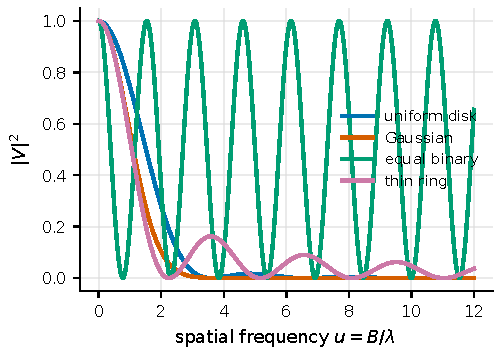
\includegraphics[width=0.88\linewidth]{figures/generated/chapter_05/ch05_vcz_visibility_models.pdf}
\caption{不同的天空亮度模型，在可见度平方 \(|V|^2\) 上留下不同的指纹。均匀圆盘出现贝塞尔型的零点，高斯源平滑衰减，等亮双星叠加一层余弦振荡，薄环则给出更密的振荡。强度干涉直接测到的正是这些曲线（的模平方），于是"读曲线"就等于"猜天空的样子"。}
\label{fig:e10-vcz-models}
\end{figure}

\section{均匀圆盘：从一条曲线量出恒星角直径}
\label{sec:e10-disk}

VCZ 定理给了通式，但天空千姿百态。要真正会用它，得从最干净的模型练手：\textbf{均匀圆盘}（uniform disk）。假设恒星是一个角直径为 \(\theta\) 的圆面，圆内表面亮度处处相等、圆外为零。这是"把恒星当成一枚均匀发光的硬币"的近似。

\textbf{推导可见度。}对圆对称的亮度分布，二维傅里叶变换退化成一维的汉克尔变换（Hankel transform）。设圆盘半径（角半径）\(a=\theta/2\)，径向空间频率 \(q=B/\lambda\)。圆对称时式 \eqref{eq:e10-vcz} 的分子写成
\[
  \int_0^{a} I_0\,J_0(2\pi q r)\,2\pi r\,\mathrm dr
  =2\pi I_0\int_0^{a}J_0(2\pi q r)\,r\,\mathrm dr,
\]
其中 \(J_0\) 是零阶贝塞尔函数（Bessel function），它是"圆对称的余弦"，正是把二维相位因子绕圆积分一圈后剩下的东西。这里用到一个标准的贝塞尔积分恒等式（任何数学物理手册都能查到）：
\[
  \int_0^{a} J_0(k r)\,r\,\mathrm dr=\frac{a}{k}\,J_1(k a),
\]
取 \(k=2\pi q\)。分母是圆盘总通量 \(I_0\cdot\pi a^2\)。两者相除：
\[
  \gamma^{(1)}
  =\frac{2\pi I_0\cdot\dfrac{a}{2\pi q}J_1(2\pi q a)}{I_0\,\pi a^2}
  =\frac{2\,J_1(2\pi q a)}{2\pi q a}.
\]
记无量纲组合 \(x\equiv 2\pi q a=2\pi\dfrac{B}{\lambda}\cdot\dfrac{\theta}{2}=\dfrac{\pi\theta B}{\lambda}\)，就得到那条著名曲线：

\begin{equation}
  V(B)=\frac{2\,J_1(x)}{x},\qquad x=\frac{\pi\,\theta\,B}{\lambda}.
  \label{eq:e10-disk}
\end{equation}
\begin{formulaexplain}
\(V(B)\)：均匀圆盘在基线 \(B\) 上的可见度。\(J_1\)：一阶贝塞尔函数。\(x=\pi\theta B/\lambda\)：无量纲"分辨程度"——越大表示星被分得越开。\(x\to0\) 时 \(2J_1(x)/x\to1\)（完全没分辨）。
\end{formulaexplain}

逐符号交代。\(V(B)\)：可见度，量纲为一，就是这条基线上的 \(\gamma^{(1)}\)（对圆盘是实数）。\(J_1(x)\)：一阶贝塞尔函数，这里我们\emph{点名引用}这个已知结果——圆形孔径的傅里叶变换总是给出 \(J_1\) 型的花样，和光学里圆孔的艾里斑（Airy pattern）同源。\(\theta\)：角直径（弧度）；\(B\)：投影基线（米）；\(\lambda\)：波长（米）。最重要的是那个组合 \(x=\pi\theta B/\lambda\)：同一颗星，基线越长或波长越短，\(x\) 越大越容易分辨；同一条基线，星越大，\(x\) 越大越敏感。

\textbf{第一零点。}曲线 \(2J_1(x)/x\) 第一次落到零，发生在 \(J_1(x)=0\) 的第一个非零根。这个根是已知的数：\(x=3.8317\)。令 \(\pi\theta B_0/\lambda=3.8317\) 解出临界基线：
\[
  B_0=\frac{3.8317}{\pi}\cdot\frac{\lambda}{\theta}=1.2197\,\frac{\lambda}{\theta}\approx1.22\,\frac{\lambda}{\theta}.
\]

\begin{equation}
  B_0\approx\frac{1.22\,\lambda}{\theta}.
  \label{eq:e10-null}
\end{equation}
\begin{formulaexplain}
\(B_0\)：可见度第一次归零的基线（米）。\(\lambda\)：波长，\(\theta\)：角直径。它标出"刚好把星分辨到第一个暗纹"所需的望远镜间距——和单口径望远镜衍射极限 \(1.22\lambda/D\) 长得一模一样，只是把口径 \(D\) 换成了基线 \(B\)。
\end{formulaexplain}

\textbf{代入真实数字。}取 VERITAS、MAGIC 常用的蓝光 \(\lambda=416\,\mathrm{nm}\)，看几种恒星大小要多长基线：
\[
  \theta=0.5\,\mathrm{mas}=0.5\times4.848\times10^{-9}\,\mathrm{rad}=2.424\times10^{-9}\,\mathrm{rad},
\]
\[
  B_0=1.22\times\frac{416\times10^{-9}}{2.424\times10^{-9}}
  =1.22\times171.6\,\mathrm{m}\approx210\,\mathrm{m}.
\]
同样地，\(\theta=1\,\mathrm{mas}\) 只要约 \(105\,\mathrm{m}\)，\(\theta=0.2\,\mathrm{mas}\) 则要约 \(520\,\mathrm{m}\)。这几个数解释了整段仪器史：Narrabri 强度干涉仪用 10--188 m 的可变基线，够测那些较亮、亚毫角秒的恒星；而要下探到几十微角秒，就得上公里级基线——这正是把大气 Cherenkov 望远镜阵列（VERITAS、MAGIC、未来的 CTAO）用作强度干涉仪的动机 \citep{1967MNRAS.137..375H,2020NatAs...4.1164A}。

\begin{figure}[tbp]
\centering
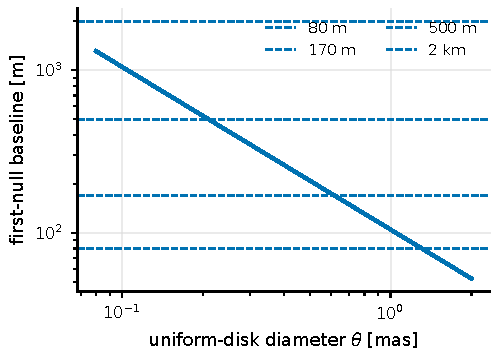
\includegraphics[width=0.86\linewidth]{figures/generated/chapter_05/ch05_uniform_disk_resolution.pdf}
\caption{均匀圆盘在 \(\lambda=416\,\mathrm{nm}\) 下的第一零点基线随角直径的变化。0.5 mas 的恒星要约 210 m 才到第一个零点，0.1 mas 量级的目标则需要公里级基线——这就是长基线 Cherenkov 阵列对蓝光强度干涉格外有吸引力的原因。}
\label{fig:e10-disk-resolution}
\end{figure}

一句实用提醒：观测时最有信息量的往往\emph{不}是零点本身，而是零点之前那段"下降区"。短基线处各种角直径的曲线几乎都贴在 \(|V|^2\approx1\)，分不出差别；零点之后 \(|V|^2\) 太低，系统误差和背景容易淹没信号；唯有下降区既有可观信号、又对 \(\theta\) 敏感。所以设计观测的第一件事，就是把目标模型的 \(|V(B)|^2\) 画出来，让基线覆盖住这段下降区（见图 \ref{fig:e10-vcz-models}）。

\section{空间 HBT：不合束，只比强度抖动同不同步}
\label{sec:e10-hbt}

到这里我们一直在谈一阶相干 \(\gamma^{(1)}\) 和复可见度——那是振幅干涉仪测的东西，需要把两束光在光学上小心地合到一起。强度干涉走的是另一条路，它连束都不合，只在探测之后比较两路\emph{强度}的抖动同不同步。凭什么这样也能测出 \(|V|\)？答案是第 \ref{chap:e08} 章的 Siegert 关系。

第 \ref{chap:e08} 章我们对同一路光、不同时刻建立了 \(g^{(2)}=1+\zeta|g^{(1)}|^2\)：热光（混沌光）的强度会成团扎堆（光子聚束），而聚束的强弱正比于一阶相干度的模平方。这条关系对"两路光、同一时刻"照样成立，只要把时间通道换成空间通道：

\begin{equation}
  g_{12}^{(2)}(0)-1=\zeta\,\big|\gamma_{12}^{(1)}\big|^2=\zeta\,\big|V(B)\big|^2 .
  \label{eq:e10-siegert}
\end{equation}
\begin{formulaexplain}
\(g_{12}^{(2)}(0)-1\)：两台望远镜零延迟强度相关的"超出量"（相对随机符合的额外扎堆）。\(\zeta\)：稀释因子（时间响应、带宽、偏振、背景一起拉低聚束高度）。\(|V(B)|^2\)：可见度模平方——正是我们想要的天体结构。
\end{formulaexplain}

逐符号说明。\(g_{12}^{(2)}(0)\)：两路强度在零时间延迟下的归一化二阶相关；减去 1，得到相对于"完全随机、毫不相关"基线的超出。\(\zeta\)（量纲为一，介于 0 和 1）：把有限探测器时间宽度、有限光学带宽、未选偏振、背景光稀释等一切"把聚束峰压平"的因素打包进来。\(|\gamma_{12}^{(1)}|^2\)：对热光/高斯混沌光，它就等于 \(|V(B)|^2\)。这条式子是空间 HBT（Hanbury Brown--Twiss）的心脏：\textbf{两台望远镜强度抖动的同步程度，直接给出可见度模平方}，全程不需要把电场合束 \citep{1956Natur.177...27B}。

\textbf{观测模型。}真机上数据分析常把式 \eqref{eq:e10-siegert} 写成一个把"仪器、背景、天体"三样东西分开的模型。其实这一步就是\emph{把式 \eqref{eq:e10-siegert} 里那个笼统的稀释因子 \(\zeta\) 拆开写清楚}——把它分成 \(\zeta=N_0\,f_1 f_2\)：\(N_0\) 收纳仪器一侧的稀释（探测器时间响应、带宽、偏振，即后面式 \eqref{eq:e10-n0} 那一项），\(f_1 f_2\) 收纳背景一侧的稀释（目标光子在两台望远镜总计数里的占比）。于是稀释因子并没有消失，只是被拆成"仪器 \(\times\) 背景"两块，各自可以单独标定：

\begin{equation}
  C_{12}(B)\equiv g_{12}^{(2)}(0)-1=N_0\,f_1 f_2\,\big|V(B)\big|^2 .
  \label{eq:e10-model}
\end{equation}
\begin{formulaexplain}
\(C_{12}\)：实测到的相关峰高度。\(N_0\)：零基线仪器响应（星没被空间分辨时应有的聚束高度）。\(f_1,f_2\)：两台望远镜里目标光子占总计数的比例。\(|V|^2\)：天体结构项。三者相乘，把仪器、背景、天空干净地拆开。
\end{formulaexplain}

逐符号：\(C_{12}(B)\) 是基线 \(B\) 上的相关峰幅度（量纲为一）；\(N_0\) 是\emph{零基线}相关幅度，即两台望远镜挨在一起、星完全没被分辨（\(|V|=1\)）时应有的聚束高度，它把探测响应后的仪器效应全收进去；\(f_1,f_2\)（量纲为一，\(\le1\)）是各台望远镜里真正来自目标的光子占比——月光、夜天光、邻星把它拉低；\(V(B)\) 是式 \eqref{eq:e10-disk}（或更复杂模型）给出的归一化可见度。这个乘积结构让分析可以逐项校准：\(|V|^2\) 随基线变，\(f_1f_2\) 随背景变，\(N_0\) 是仪器的"身份证"。

\textbf{零基线幅度有多小。}对未选偏振的热光，若探测器有效时间宽度为 \(\Delta t_{\rm eff}\)、光学带宽为 \(\Delta\nu\)，零基线幅度的数量级是

\begin{equation}
  N_0\sim\frac{1}{2\,\Delta\nu\,\Delta t_{\rm eff}},\qquad
  \Delta\nu\simeq\frac{c\,\Delta\lambda}{\lambda^2}.
  \label{eq:e10-n0}
\end{equation}
\begin{formulaexplain}
\(N_0\)：星未被分辨时的聚束峰高度。\(\Delta\nu\)：光学频率带宽（Hz）。\(\Delta t_{\rm eff}\)：电子学有效时间宽度（s）。分母里的 \(2\) 是未选偏振（两个偏振模式）带来的稀释。带宽越宽、时间响应越慢，热光聚束峰被平均得越低。
\end{formulaexplain}

物理上这很好理解（可回想第 \ref{chap:e02} 章带宽与相干时间互为倒数）：聚束这件事只在一个相干时间 \(\tau_c\sim1/\Delta\nu\) 之内才"看得见"，而探测器要花 \(\Delta t_{\rm eff}\) 去积分。探测器远慢于相干时间时（\(\Delta t_{\rm eff}\gg\tau_c\)），一次积分里塞进了 \(\sim\Delta t_{\rm eff}/\tau_c=\Delta\nu\,\Delta t_{\rm eff}\) 个互不相关的相干块，聚束信号被这么多块一平均就摊薄了，于是 \(N_0\) 反比于这个大数。

\textbf{代入 VERITAS 的真实参数}（\(\lambda=416\,\mathrm{nm}\)、\(\Delta\lambda=13\,\mathrm{nm}\)、\(\Delta t_{\rm eff}\sim4\,\mathrm{ns}\)）：先算带宽
\[
  \Delta\nu\simeq\frac{c\,\Delta\lambda}{\lambda^2}
  =\frac{(3\times10^8)\,(13\times10^{-9})}{(416\times10^{-9})^2}
  =\frac{3.9}{1.73\times10^{-13}}\ \mathrm{Hz}\approx2.3\times10^{13}\,\mathrm{Hz},
\]
再代进 \(N_0\)：
\[
  N_0\sim\frac{1}{2\,(2.3\times10^{13})\,(4\times10^{-9})}
  =\frac{1}{1.8\times10^{5}}\approx5\times10^{-6}.
\]
数量级是百万分之几。真机拟合得到的 \(N_0\approx1.25\times10^{-6}\)，比粗估略低——因为真实的滤光片形状、电子响应和系统效率还要再把峰压一压。无论如何，结论令人肃然：\textbf{热光的聚束峰只有百万分之一量级}，要在这么低的信号上量恒星，靠的是长时间积累和对 \(N_0\) 的严苛标定（图 \ref{fig:e10-zero-baseline}）\citep{2020NatAs...4.1164A}。

\begin{figure}[tbp]
\centering
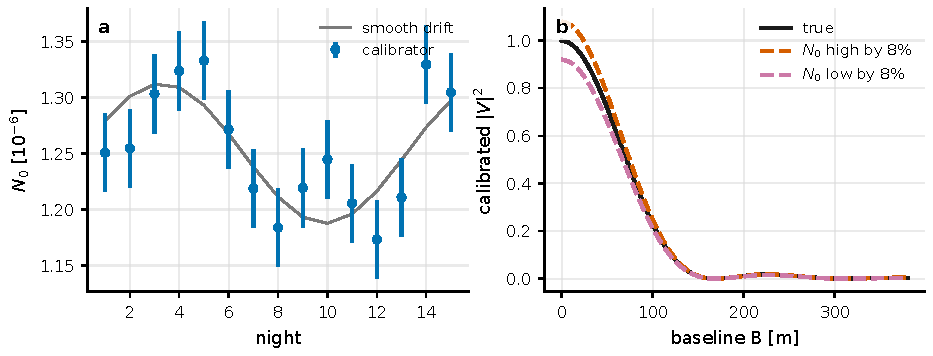
\includegraphics[width=0.92\linewidth]{figures/generated/chapter_05/ch05_zero_baseline_calibration.pdf}
\caption{零基线幅度 \(N_0\) 的标定会直接搬运到 \(|V|^2\) 上。左：校准星给出的夜间 \(N_0\) 漂移。右：\(N_0\) 若偏高或偏低 8\%，\emph{所有}基线上的 \(|V|^2\) 都被整体拉伸，进而把角直径、边缘昏暗或扁率的拟合推向错误值。这解释了为什么 \(N_0\) 是强度干涉里最要命的一项系统。}
\label{fig:e10-zero-baseline}
\end{figure}

\section{相位缺失：软肋，也是护身符}
\label{sec:e10-phase}

强度干涉只测 \(|V|^2\)——式 \eqref{eq:e10-model} 里那个模平方——把复可见度 \(\gamma_{12}^{(1)}\) 的辐角（傅里叶相位）扔掉了。这带来一个原理性的模糊。

\textbf{镜像退化。}考虑一幅亮度分布 \(I(l,m)\) 和它绕中心翻转后的镜像 \(I(-l,-m)\)。用式 \eqref{eq:e10-vcz} 做傅里叶变换，实亮度分布的傅里叶变换满足 \(\gamma(-u,-v)=\gamma^{\ast}(u,v)\)（因为 \(I\) 是实的）；而镜像分布的傅里叶变换恰好是原来那个的复共轭。取模平方时，复共轭不改变模，于是
\[
  \big|V_{\text{原图}}(u,v)\big|^2=\big|V_{\text{镜像}}(u,v)\big|^2 .
\]
两幅长得不一样的天空，给出\emph{完全相同}的 \(|V|^2\)——只测模平方的仪器无法区分它们（图 \ref{fig:e10-phase-ambiguity}）。这就是为什么"从 \(|V|^2\) 直接成像"是一件需要额外信息（二维 \(u,v\) 覆盖、物理先验、三阶相关或相位恢复算法）的难事，我们把真正的成像留到第 \ref{chap:e11} 章。

\begin{figure}[tbp]
\centering
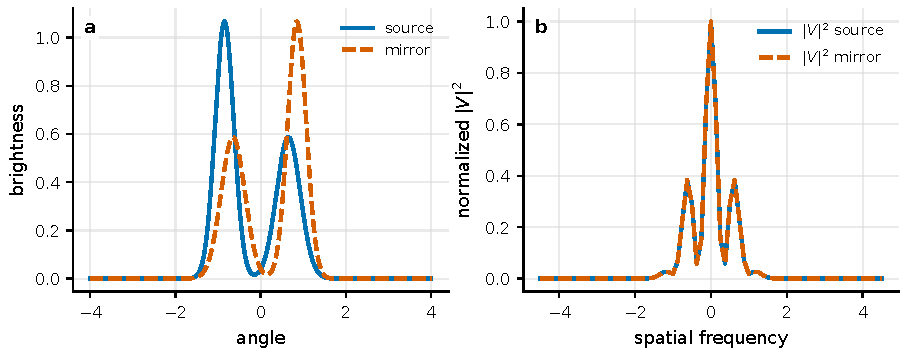
\includegraphics[width=0.92\linewidth]{figures/generated/chapter_05/ch05_phase_ambiguity.pdf}
\caption{只测 \(|V|^2\) 会丢掉傅里叶相位。左：一个源和它的镜像源，亮度分布明显不同。右：两者的 \(|V|^2\) 完全重合。强度干涉要成像，必须靠二维 \(u,v\) 覆盖、物理先验、三阶（闭合）相关或相位恢复算法来打破这类退化。}
\label{fig:e10-phase-ambiguity}
\end{figure}

\textbf{丢相位换来了什么？}答案是：对光程和大气抖动近乎免疫——这正是让 Cherenkov 望远镜能做干涉的根本原因。振幅干涉仪要把两束光在光学上合到一起看条纹，必须把两条光路的\emph{光程}稳定到波长的一小部分（几十纳米量级）；而大气湍流让波前不停地起伏，给每台望远镜叠加一个随机的、快速跳动的光程偏移，术语叫\textbf{活塞相位}（piston）。piston 对振幅干涉是致命的，条纹会被抖没。

强度干涉却几乎不在乎它。理由在于：它比较的是两路\emph{强度}的抖动同不同步，只需要把两路\emph{电子信号}在时间上对齐到探测响应时间的一小部分即可。对 \(1\,\mathrm{GHz}\) 电子带宽，时间分辨约 1 ns，对应的光程容差是 \(c\times1\,\mathrm{ns}\approx30\,\mathrm{cm}\)——要几厘米到几十厘米的路径误差才会明显降低相关。大气 piston 那点纳米到微米量级的光程抖动，落在这个容差里连零头都算不上。换句话说，\textbf{强度干涉用"丢掉相位"这个代价，买来了"不怕大气、不需精密光程"这个巨大便利}。正因如此，那些光学像质远达不到专业干涉仪水准、却拥有大口径和快探测器的 Cherenkov 望远镜，反而成了理想的强度干涉阵列 \citep{2006ApJ...649..399L,2024MNRAS.529.4387A}。

\section{本章要点}
\label{sec:e10-summary}

\begin{itemize}
  \item \textbf{几何定角尺度。}投影基线 \(\bm B_\perp\) 给程差 \(\bm B\cdot\bm s\)，空间频率 \(u=B_x/\lambda,\ v=B_y/\lambda\) 是无量纲的"波长数"。百米基线、蓝绿光对应约 1 mas（\(B/\lambda=2\times10^8\)，倒过来 \(\lambda/B\approx1\,\mathrm{mas}\)）。分辨本领由基线、而非口径决定。
  \item \textbf{相干度是一支复箭头。}一阶空间相干度 \(\gamma_{12}^{(1)}=\langle E_1^\ast E_2\rangle/\sqrt{\langle|E_1|^2\rangle\langle|E_2|^2\rangle}\)：模给相干强弱，辐角给傅里叶相位。
  \item \textbf{van Cittert--Zernike 定理。}非相干远场源的 \(\gamma^{(1)}(u,v)\) 就是归一化天空亮度的傅里叶分量（式 \eqref{eq:e10-vcz}）。短基线看粗结构、长基线看细结构。成立要四条：源内非相干、窄带、小视场、源不变。
  \item \textbf{均匀圆盘。}\(V(B)=2J_1(x)/x,\ x=\pi\theta B/\lambda\)（一阶贝塞尔函数）；第一零点 \(x=3.8317\) 给 \(B_0\approx1.22\lambda/\theta\)。416 nm、0.5 mas \(\Rightarrow\) 约 210 m。最有信息的是零点前的下降区。
  \item \textbf{空间 HBT。}把第 \ref{chap:e08} 章 Siegert 关系搬到空间通道：\(g_{12}^{(2)}(0)-1=\zeta|V(B)|^2\)；不合束、只比强度抖动同步度就能测 \(|V|^2\)。观测模型 \(C_{12}=N_0 f_1 f_2|V|^2\)，零基线幅度 \(N_0\sim1/(2\Delta\nu\Delta t_{\rm eff})\)；VERITAS 参数给约 \(5\times10^{-6}\)，实测 \(1.25\times10^{-6}\)。
  \item \textbf{相位缺失是双刃剑。}只测 \(|V|^2\)，镜像亮度分布 \(I(-l,-m)\) 给同样的 \(|V|^2\)（退化）；但代价换来对光程/大气 piston 的免疫——这正是 Cherenkov 望远镜能做干涉的原因。成像留到第 \ref{chap:e11} 章。
\end{itemize}

\medskip
\noindent\textbf{想一想。}
\begin{itemize}
  \item 若把观测波长从 416 nm 换成 640 nm 的红光，同一颗 0.5 mas 恒星的第一零点基线会变长还是变短？变到多少米？
  \item 两台望远镜里目标光子占比若从 70\% 掉到 50\%，式 \eqref{eq:e10-model} 里的相关峰会被压到原来的几分之几？要恢复同样显著性，积分时间大致要加多少倍（回想 SNR 随时间只按平方根增长）？
  \item 为什么"窄带"是 VCZ 定理的必要条件？如果带宽很宽，式 \eqref{eq:e10-uv} 会出什么问题？
\end{itemize}
